\documentclass[a4paper]{article}
\usepackage[a4paper, margin=2.5cm]{geometry}
\usepackage[utf8]{inputenc}
\usepackage[T1]{fontenc}
\usepackage{graphicx}
\usepackage[english]{babel}
\usepackage{hyperref}
\usepackage{float}
\usepackage{amsthm}
\usepackage{amsmath}
\usepackage{multicol}
\usepackage{wrapfig}
\usepackage{bm}
\usepackage{amssymb}
\usepackage{listings}
\usepackage{minted}
\usepackage{tikz}
\usetikzlibrary{calc,arrows.meta,positioning, automata, shapes}
\usepackage[]{algorithm2e}
\usepackage{paralist}

\hypersetup{
    colorlinks = true,
    citecolor = black,
    urlcolor = blue,
    linkcolor = black,
}
\usepackage[
    backend=biber,
    style=alphabetic,
    citestyle=authoryear
]{biblatex}
\usepackage{csquotes}
\addbibresource{ref.bib}

\newcommand{\question}[2]{
\paragraph{Question #1} -- \textit{#2}

}
\newcommand{\programming}[1]{
\paragraph{Programming} -- \textit{#1}

}

\title{Reinforcement Learning Lab Session 6}
\author{Your Name Here}
 
\begin{document}
\maketitle
\section*{General Information}
This lab session will cover all the Reinforcement Learning material from courses 1 to 4. It will be graded lab sessions. You are free to use any content you want regarding the questions, but please refrain from using outside code beyond the previous lab sessions.

It should be doable in 4 hours, but the deadline will be set to Sunday 29th. As usual, for there on, each day of delay will remove 2.5/10 points from your grade.

\paragraph{Submission} --
You will have to submit both a report and code through Blackboard. Use the code available on the git at \url{http://github.com/Louis-Bagot/RL_Lab/lab_session6} or \url{https://github.com/Rajawat23/RL_Lab/lab_session6}.

Make a copy of this LaTeX document from folder \textbf{report}, and fill it according to the instructions below. Please to not alter this base document, only add your content.

\question{}{Questions will look like this. For questions, write the answer just below where the (your answer here) appears.}
\programming{Programming exercises will look like this. For programming exercises, read the \texttt{instructions.md} of the corresponding section, and then fill in the corresponding TODO flags in the code. If this text asks for a plot, copy the plot output of your code in the document, in the figure space provided (in addition to leaving it in the plots folder in the code). If the text asks for an explanation of the results, write it as you would answer a question.}

\tableofcontents
\newpage

\section{Bandits}
\question{1}{Explain, in a few lines, the k-armed Bandit problem. Give an example of a real-world application, detailing actions and rewards.}
(your answer here)

\question{2}{Derive the incremental updates of the Sample 
Average method.}
(your answer here)


\question{3}{Explain, with your own words, the difference between Sample Average and Weighted Average methods}
(your answer here)

\question{4}{Explain the impact of the hyper-parameters of the following algorithms: $\epsilon$ in $\epsilon$-greedy, $c$ in UCB, and $\alpha$ in Gradient Bandit. Use extreme values as examples.}
(your answer here)

\question{5}{Show that the Sample Average method erases the bias introduced by the initialization of the $Q$ estimates. What does this mean for Optimistic Greedy? Show that, despite this, Optimistic Greedy does not work on non-stationary problems.}
(your answer here)

\programming{Implement a Sample Average and Weighted Average version of $\epsilon$ greedy on a Non-Stationary k-armed Bandit problem. In order to see results, run the experiment for $10k$ steps, and paste here the resulting performance plot in the Figure \ref{fig:sa_vs_wa} below. Explain your results below.}
(your explanation here)
\begin{figure}[H]
    \centering
    % Change the plot name here:
    
\includegraphics[width=8cm]{plots/your_plot_here.png}
    \caption{Comparison: $\epsilon$-greedy algorithm with Sample Average versus Weighted Average updates.}
    \label{fig:sa_vs_wa}
\end{figure}{}


\section{Markov Decision Processes}
For questions where a drawing (MDP or diagram) is required, you can use whichever of the following methods:
\begin{itemize}
    \item a (properly cropped and clear) photo of a drawing on paper. Make sure everything is readable.
    \item a tikz diagram, i.e. the plotting tool for LaTeX (if you know how it works. Don't learn for this report otherwise, tikz takes an eternity)
    \item \href{www.mathcha.io}{Mathcha}, which can generate tikz or pngs. (recommended)
\end{itemize}{}

\question{1}{Define a Markov Decision Process, and the goal of the Reinforcement Learning problem.}
(your answer here)

\question{2}{Show that the MDP framework generalizes over Bandits by drawing the Bandits problem as a MDP with reward distributions $r_a$ for each action $a$. Paste your drawing on Figure \ref{fig:bandit_mdp}. Shortly explain your submission.}

\begin{figure}[H]
    \centering
    % Change the plot name here:
    
\includegraphics[width=8cm]{plots/your_plot_here.png}
    \caption{The MDP corresponding to the Bandit problem with reward distributions $r_a$, $\forall$ actions $a$}.
    \label{fig:bandit_mdp}
\end{figure}{}
(your explanation here)


\question{3}{Turn the following statement into a MDP, with states and transitions with actions (named), probabilities and rewards. Paste the graph on Figure \ref{fig:q3}; pick real values for both rewards and probabilities (no unknowns). Shortly explain your submission after the statement and plot.}

Statement:

\texttt{You go to the university using Velo -- Antwerp's shared bikes. There are three stations where you can drop off your bike on the way: the park, furthest from the university; the cemetery, second furthest; and the university station, right in front of your destination.
You want to take the least time possible to go to the university, and you take much longer walking than biking. \\
At any station, you can either decide to drop off your bike and walk to the university, or continue to the next station.
However, it sometimes happens that the stations are full - you cannot drop off your bike there. You can either go back, or, if possible, continue.\\
You notice that the amount of free spots in the first stations often aligns with the amount of free spots in the following stations - or is less. In order to decide whether you should drop off your bike or not, you take note of the last station's number of free spots - it can either be a lot, or a few, or none.\\
When you have to go back, we assume that people could've come to pick or drop bikes, so the transition doesn't depend on the previous state of the station.
}

\begin{figure}[H]
    \centering
    % Change the plot name here:
    
\includegraphics[width=8cm]{plots/your_plot_here.png}
    \caption{The MDP corresponding to the statement of Question 3}.
    \label{fig:q3}
\end{figure}{}
(your explanation here)

\question{4}{RL has been widely popular lately because of its combination with Deep Learning (using Neural Nets as policy or value function approximators), leading to incredible performances on difficult environments like video games. One such game is the first Mario World. Show how the MDP can look like for the frames of the game. Where can stochasticity be involved?}


\section{Control}
In lab session 2 and 3, the Value Iteration algorithm was stopped after a maximum number of iterations. However, this is not the natural stopping condition of the algorithm: it should stop when the value estimates have converged: $V_k = v*$. When implementing this, we define convergence of the $V_{k-1},V_k,V_{k+1}..$ stream of vector values as $$ \vert\vert V_{k+1} - V_k \vert\vert_2 < \delta $$
Where $\delta$ is an arbitrary small constant ($\delta = 0.01$ in the code). The number of iterations of Value Iteration to convergence is a measure of the algorithm's performance.\\

Policy Iteration alternates evaluating a policy $\pi$ until convergence to $V_\pi$, and updating the policy to be greedy over the new values, $\pi ^\prime = greedy(v_\pi)$. We define \textit{convergence in policy} as  $\pi^\prime = \pi$ (same action in all states), and \textit{convergence in value} as $$ \vert\vert V_{\pi ^\prime} - V_\pi \vert\vert_2 < \delta $$

Value Iteration only converges in value, as there is no explicit policy. When comparing convergence speed in value of Value Iteration vs Policy Iteration, make sure to compare the number of single sweeps over the state space! (iterations)

\programming{Implement Value Iteration on the course's diamond/pit Gridworld environment (course and Lab session 2). You can reuse Environment code from before.}

\programming{Implement Policy Iteration on the course's diamond/pit Gridworld environment.}

\question{1}{Discuss and compare the performances of both algorithms. Under what circumstances can one come on top of the other?}

\question{3}{Explain the fundamental differences between QLearning and the Value Iteration / Policy Iteration algorithms. Can you see why QLearning is more interesting in the general case?}

\section{Bonus}
\programming{\textbf{BONUS, 1.5pts} Implement the Gridworld drawn on Figure \ref{fig:river_crossing}: a river crossing. The actions are up, down, left, right and "do nothing". The agent needs to cross a river from the lower left corner (state S) to the upper right corner (state G). This $3\times 5$ Gridworld is divided on the 2nd row by a river that might push the agent right upon entering by one, two or three squares, with corresponding probabilities $0.2, 0.5$ and $0.3$. If the agent is pushed off to the far right in the river, the episode ends with reward $-1$. If the agent reaches the goal, the reward is $+1$. Note that it is the transition to the state (i.e. "right" from (0,3) to G=(0,4)) that yields the reward, and states G and red (1,4) are terminal. }

\begin{figure}[H]
    \centering
    % Change the plot name here:
    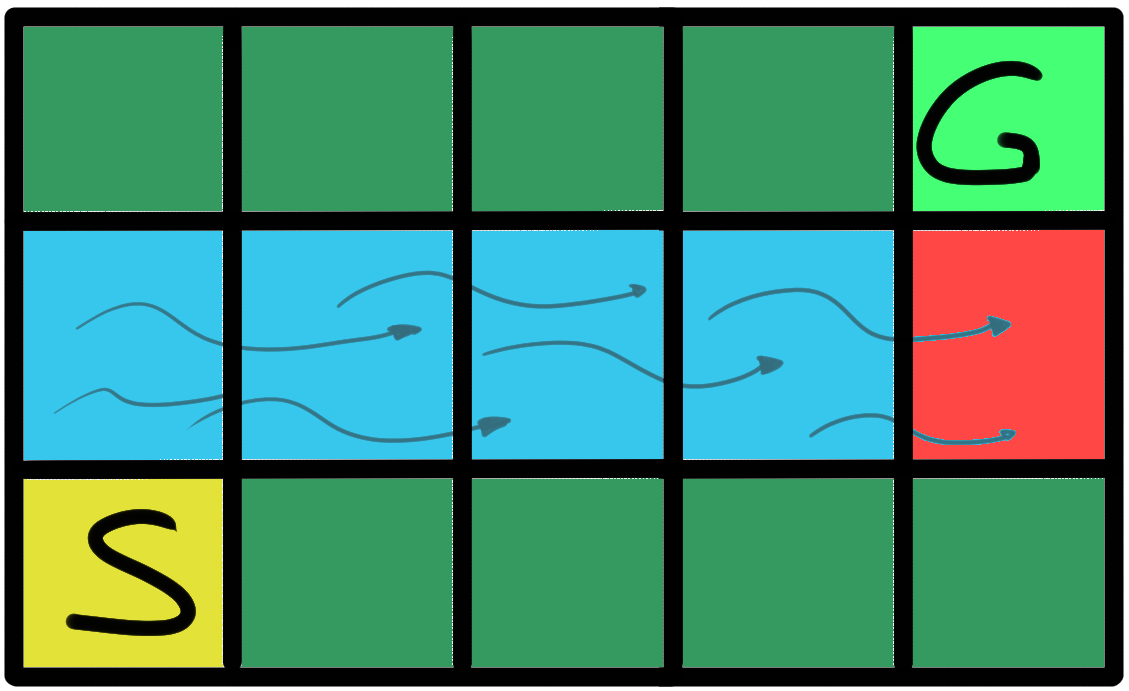
\includegraphics[width=6cm]{plots/river.png}
    \caption{The River Crossing MDP}.
    \label{fig:river_crossing}
\end{figure}{}


\printbibliography
\end{document}

